%!TEX root = ../../architekturdokumentation.tex
\chapter{Technologische Übersicht}
	\begin{wrapfigure}[10]{R}{0.5\textwidth}
  		\vspace{-25pt}
	  	\begin{center}
    		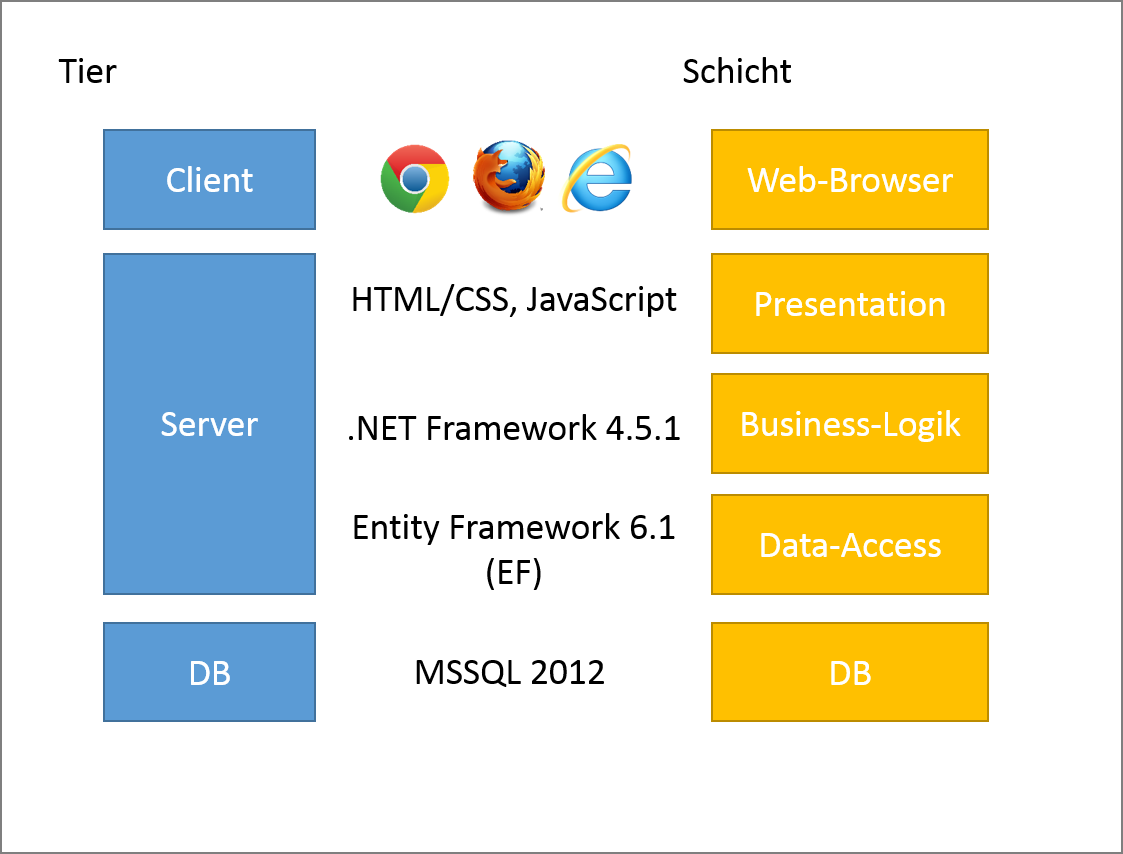
\includegraphics[height=7cm]{content/architekturdokumentation/images/technologische_uebersicht.png}
	  	\end{center}
  		\vspace{-20pt}
	 	\caption{Technologische Übersicht}
	\end{wrapfigure}
    Diese Darstellung soll als Big-Picture üder die verwendeten Technologien nach Tier dienen.
    An die Client-Tier wird nebst dem Browser keine spezielle Anforderung gestellt.
  	Server-seitig wird das .NET Framework 4.5.1 verwendet. Der Datenbankzugriff zur Datenbank wird durch das Entity Framework 6.1 ermöglicht. Das Entity Framework ermöglicht eigentlich ein austauschbares Datenbanksystem. Für das Projekt haben wir uns aber für den Einsatz von MSSQL entschieden.
  	\vspace{1.5cm}

	\section{Übersicht der Komponenten}
	Die Abbildung zeigt eine Übersicht über die einzelnen Komponenten des Systems. Sichtbar ist auch die Kommunikation der Services mit den Schnittstellen.
    \begin{figure}[h]
  		\vspace{-5pt}
    	\centering
    	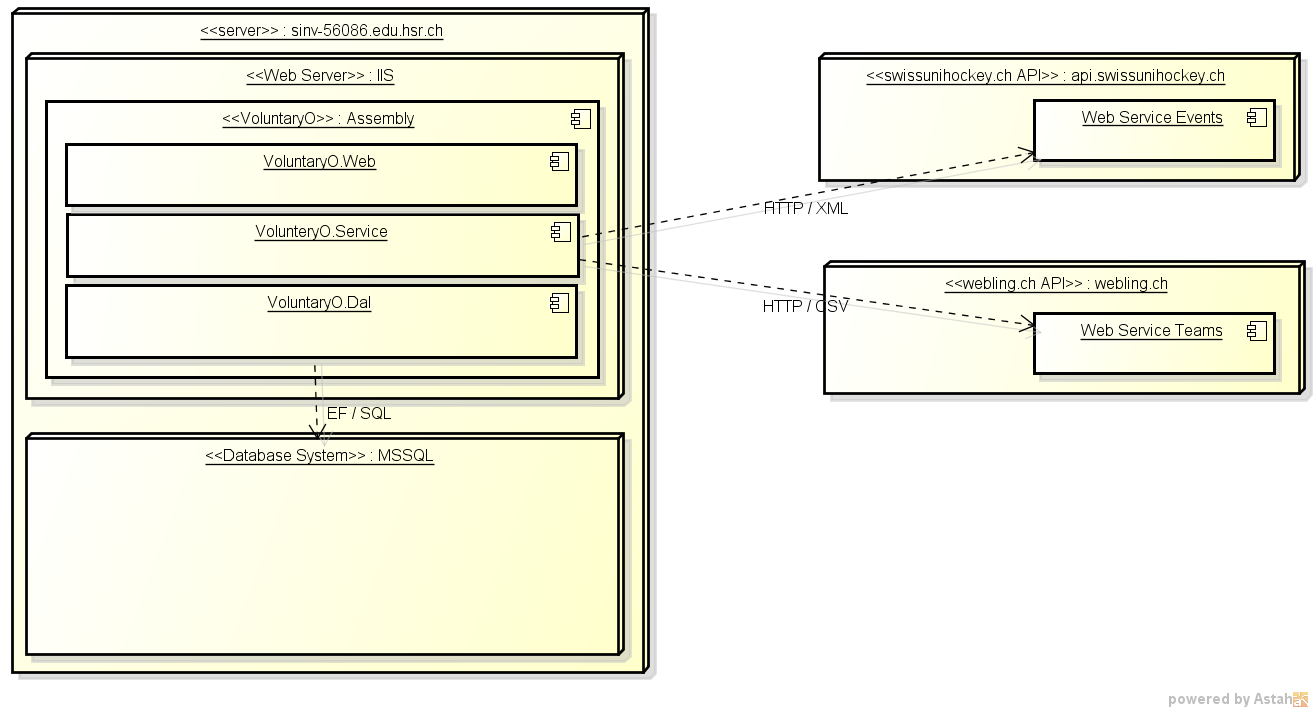
\includegraphics[width=0.9\textwidth]{content/architekturdokumentation/images/uebersicht_der_komponenten.png}
  		\vspace{-25pt}
    	\caption{Übersicht der Komponenten}
	\end{figure}
	